\section{Neural Networks}\label{sec:ch2:nns}
\subsection{The Neuron and Single-Layer Neural Networks}

\begin{figure}
  \centering
  % \pagestyle{empty}

\def\layersep{2.5cm}

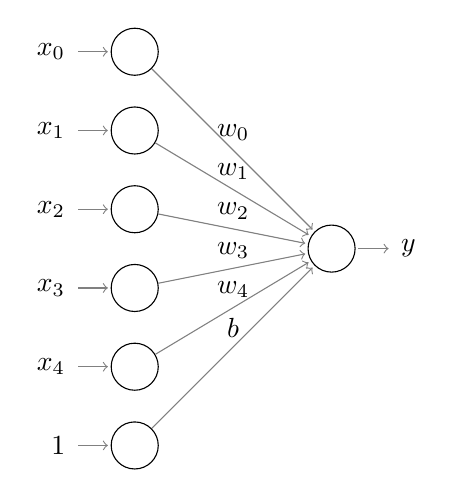
\begin{tikzpicture}[shorten >=1pt,->,draw=black!50, node distance=\layersep]
    \tikzstyle{every pin edge}=[<-,shorten <=1pt]
    \tikzstyle{neuron}=[circle,draw=black,minimum size=17pt,inner sep=0pt]
    \tikzstyle{input neuron}=[neuron];
    \tikzstyle{output neuron}=[neuron, fill=red!50];
    \tikzstyle{hidden neuron}=[neuron];
    \tikzstyle{annot} = [text width=4em, text centered]

    % Draw the input layer nodes
    \foreach \name / \y in {0,...,4}
    % This is the same as writing \foreach \name / \y in {1/1,2/2,3/3,4/4}
        \node[input neuron,pin=left:$x_\y$] (I-\name) at (0,-\y) {};
    \node[input neuron,pin=left:1] (I-5) at (0,-5) {};

    % Draw the output layer node
    \node[hidden neuron,pin={[pin edge={->}]right:$y$}] (O) at (\layersep, -2.5) {};

    % Connect every node in the input layer with every node in the
    % hidden layer.
    % \foreach \source in {1,...,5}
        % \draw(I-\source) edge (O) node[above, midway] {$w_\source$};
    \foreach \source in {0,...,4}
        \draw[->] (I-\source) -- (O) node[above,midway] {$w_\source$};
    \draw[->] (I-5) -- (O) node[above,midway] {$b$};

    % Annotate the layers
    % \node[annot,above of=I-1, node distance=1cm] (il) {Input Layer};
    % \node[annot,right of=hl] {Output layer};
\end{tikzpicture}
% End of code

  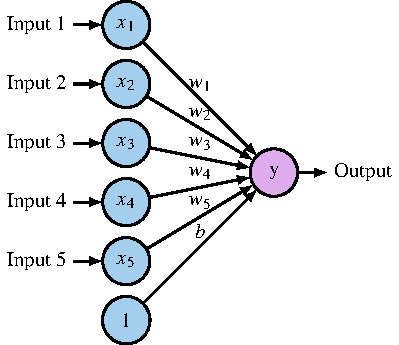
\includegraphics{\imgpath/singlelayer.pdf}
  \mycaption{A single neuron}{The neuron is composed of inputs $x_i$, weights
    $w_i$ (and a bias term), as well as an activation function. Typical activation
    functions include the sigmoid function, tanh function and the ReLU}
  \label{fig:ch2:singlelayer}
\end{figure}

The neuron, shown in \autoref{fig:ch2:singlelayer} is the core building block of
neural networks. It takes the dot product between an input vector $\vec{x} \in
\reals[D]$ and a weight vector $\vec{w}$, before applying a chosen nonlinearity.
Historically, the sigmoid nonlinearity was the most popular but today other
functions have become more popular. Still, the convention has remained to name this
generic nonlinearity $\sigma$. I.e.
%
\begin{equation}
  y = \sigma(\langle\vec{x}, \vec{w}\rangle) = \sigma\left(\sum_{i=0}^{D} x_i w_i \right)
\end{equation}
%
where we have used the shorthand $b=w_0$ and $x_0 = 1$. Also, note that we will
use the common practice in the neural network literature to call the parameters
\emph{weights} denoted by $w$.

Some of the other popular nonlinear functions $\sigma$ are
the tanh and ReLU:
\begin{align}
  \F{tanh}(x) &= \frac{e^{x} - e^{-x}}{e^{x} + e^{-x}} \label{eq:ch2:tanh}\\
  \F{ReLU}(x) &= \max (x, 0) \label{eq:ch2:relu}
\end{align}
%
See \autoref{fig:ch2:nonlinearities} for plots of these. The original Rosenblatt
perceptron \cite{rosenblatt_perceptron:_1958} also used the Heaviside function
$\F{H}(x) = \mathbb{I}(x > 0)$. % The sigmoid nonlinearity
% naturally arises when we want to do classification with class labels $\{0,1\}$,
% as does the tanh function for classification with class labels $\{-1, 1\}$. The
% ReLU however is used more often in deeper architectures
% \cite{nair_rectified_2010}.

Note that if $\langle\vec{w}, \vec{w}\rangle = 1$ then $\langle\vec{x},
\vec{w}\rangle$ is the distance from the point $\vec{x}$ to the hyperplane with
normal $\vec{w}$ (with non-unit-norm $\vec{w}$, this can be thought of as a scaled
distance). Thus, the weight vector $\vec{w}$ defines a hyperplane in $\reals[D]$
which splits the space into two. The choice of nonlinearity then affects how
points on each side of the plane are treated. For a sigmoid, points far below
the plane get mapped to 0 and points far above the plane get mapped to 1 (with
points near the plane having a value of 0.5). For tanh nonlinearities, these
points get mapped to -1 and 1. For ReLU nonlinearities, every point below the
plane ($\langle\vec{x}, \vec{w}\rangle < 0$) gets mapped to zero and every point
above the plane keeps its inner product value.

Nearly all modern neural networks use the ReLU nonlinearity and it has
been credited with being a key reason for the recent surge in deep learning
success \cite{glorot_deep_2011, nair_rectified_2010}. In particular:
\begin{enumerate}
\item It is less sensitive to initial conditions as the gradients that
  backpropagate through it will be large even if $x$ is large. A common
  observation of sigmoid and tanh nonlinearities was that their learning would
  be slow for quite some time until the neurons came out of saturation, and then
  their accuracy would increase rapidly before levelling out again at
  a minimum~\cite{glorot_understanding_2010}. The ReLU, on the other hand, has
  a constant gradient when it is activated.
\item It promotes sparsity in outputs, by setting them to a hard 0. Studies
  on brain energy expenditure suggest that neurons encode information in
  a sparse manner. \cite{lennie_cost_2003} estimates the percentage of
  neurons active at the same time to be between 1 and 4\%. Sigmoid and tanh
  functions will typically have \emph{all} neurons firing, while
  the ReLU can allow neurons to fully turn off.
\end{enumerate}

\begin{figure}
    \qquad
    % \section{Wavelet-Based Nonlinearities}\label{sec:ch6:nonlinearities}
Returning to the goals from \autoref{sec:ch6:learning}, the experiments from the
previous section have shown that while it is possible to use a wavelet gain
layer ($G$) in place of a convolutional layer ($H$), this may come with a small
performance penalty. Ignoring this effect for the moment, in this section, we
continue with our investigations into learning in the wavelet domain. In
particular, is it possible to replace a pixel domain nonlinearity $\sigma$ with
a wavelet-based one $\sigma_w$?

But what sensible nonlinearity should be used? Two particular options are good initial
candidates:
\begin{enumerate}
  \item The ReLU: this is a mainstay of most modern neural networks and has
    proved invaluable in the pixel domain. Its pseudo-nonlinearity
    ($\F{ReLU}(Ax) = A\F{ReLU}(x)$) makes learning less dependent on signal
    amplitudes. Perhaps its sparsifying
    properties will work well on wavelet coefficients too. 
  \item Thresholding: a technique commonly applied to wavelet
    coefficients for denoising and compression. Many proponents of compressed
    sensing and dictionary learning even like to compare soft thresholding to a
    two-sided ReLU \cite{papyan_theoretical_2018, papyan_convolutional_2017-1}.
\end{enumerate}

In this section, we will look at both and see if they improve the gain
layer. If they do, it would the be possible to connect multiple layers in the
wavelet domain, avoiding the necessity to do inverse wavelet transforms after
learning.

\subsection{ReLUs in the Wavelet Domain}
Applying the ReLU to the real lowpass coefficients is not difficult, but it does
not generalize so easily to complex coefficients. The simplest option is to apply
it independently to the real and imaginary coefficients, effectively only
selecting one quadrant of the complex plane:
\begin{align}
  u_{lp} &= \F{max}(0,\ v_{lp}) \\
  u_{j} &= \F{max}(0,\ \real{v_{j}}) + j\F{max}(0,\ \imag{v_j}) \label{eq:ch6:relu_bp}
\end{align}

Another option is to apply it to the magnitude of the bandpass coefficients. Of
course, these are all strictly positive so the ReLU on its own would not do
anything. However, they can be arbitrarily scaled and shifted by using a batch
normalization layer. Then the magnitude could shift to (invalid) negative
values, which can then be rectified by the ReLU.

Dropping the scale subscript $j$ for clarity (we need it for the square root of 
negative 1), let a bandpass coefficient at a given scale be
$v = r_v e^{j\theta_v}$ and define
$\mu_r = \mathbb{E}[r_v]$ and $\sigma_r^2 = \mathbb{E}[(r_v-\mu_r)^2]$, then
applying batch-normalization and the ReLU to the magnitude of $v_j$ means we
get:
\begin{align}
  r_u &= \F{ReLU}(BN(r_v)) = \max(0,\ \gamma \frac{r_v-\mu_r}{\sigma_r} + \beta) \label{eq:ch6:magrelu_bp} \\
  u &= r_u e^{j\theta_v} \label{eq:ch6:magrelu_bp2}
\end{align}
This also works equivalently on the lowpass coefficients, although $v_{lp}$ can
be negative unlike $r_v$:
\begin{equation}
  u_{lp} = \F{ReLU}(BN(v_{lp})) = \max(0, \gamma' \frac{v_{lp} - \mu_{lp}}{\sigma_{lp}} + \beta') \label{eq:ch6:bnrelu_lp}
\end{equation}
%
\subsection{Thresholding}
For $t \in \reals$ and $z = re^{j\theta} \in \complexes$ the pointwise hard thresholding is:
\begin{align}
  \mathcal{H}(z, t) &= \left\{ \begin{array}{ll}
    z & r \geq t \\
    0 & r < t\\
  \end{array} \right. \\
  &= \indic(r > t) z
\end{align}
and the pointwise soft thresholding is:
\begin{align}
  \mathcal{S}(z, t) &= \left\{ \begin{array}{ll}
    (r-t)e^{j\theta} & r \geq t \\
    0 & r < t\\
  \end{array} \right. \\
  &= \max(0, r - t)e^{j\theta} \label{eq:ch6:relu_st}
\end{align}
Note that \eqref{eq:ch6:relu_st} is very similar to \eqref{eq:ch6:magrelu_bp} and \eqref{eq:ch6:magrelu_bp2}.
We can rewrite \eqref{eq:ch6:magrelu_bp} by taking the strictly positive terms
$\gamma$, $\sigma$ outside of the $\max$ operator:
\begin{align}
  r_u &= \max(0, \gamma \frac{r_v-\mu_r}{\sigma_r} + \beta) \\
      &= \frac{\gamma}{\sigma_r}\max\left(0, r_v - \left(\mu_r - \frac{\sigma_r\beta}{\gamma}\right)\right) \label{eq:ch6:bnrelu_soft}
\end{align}
then if $t' = \mu_v - \frac{\sigma_r\beta}{\gamma} > 0$, \textbf{doing batch
normalization followed by a ReLU on the magnitude of the complex coefficients is the
same as soft shrinkage with threshold $t'$, scaled by a factor
$\frac{\gamma}{\sigma_r}$}.

The same analogy does not apply to the lowpass
coefficients, as $v_{lp}$ is not strictly positive.

While soft thresholding is similar to batch normalizations and ReLUs, we would also like
to test how well it performs as a sparsity-inducing wavelet nonlinearity.
To do this, we can:
\begin{itemize}
  \item Learn the threshold $t$
  \item Adapt $t$ as a function of the distribution of activations to achieve a desired sparsity level.
\end{itemize}
In early experiments, we found that trying to set
desired sparsity levels by tracking the standard deviation of the statistics
and setting a threshold as a function of it performed very poorly (causing a
drop in top-1 accuracy of at least 10\%).
Instead, we choose to learn a threshold $t$. We make this an unconstrained
optimization problem by changing \eqref{eq:ch6:relu_st} to:
\begin{equation}
  \mathcal{S}(v, t) = \max(0, r-|t|)e^{j\theta}  \label{eq:ch6:relu_st2}
\end{equation}

Learning a threshold is only possible for soft thresholding, as $\dydx{L}{t}$ is
not defined for hard thresholding. Like batch normalization, we learn
independent thresholds $t$ for each channel.

    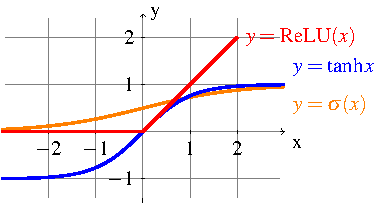
\includegraphics{\imgpath/nonlinearities.pdf}
    \quad
    % 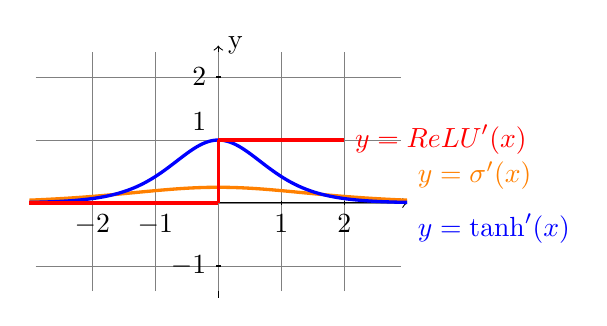
\begin{tikzpicture}[scale=0.8]
  % Draw axes
  \draw[->] (-3,0) -- (3,0);
  \draw[->] (0,-1.5) -- (0,2.5) node[right] {y};

  % Draw gridlines
  \draw[step=1cm,gray,very thin] (-2.9,-1.4) grid (2.9, 2.4);

  \foreach \x in {-2,-1,1,2}
    \draw (\x cm,1pt) -- (\x cm,-1pt) node[anchor=north] {$\x$};
  \foreach \y in {-1,  2}
    \draw (1pt, \y cm) -- (-1pt, \y cm) node[anchor=east] {$\y$};
  \draw (1pt, 1 cm) -- (-1pt, 1 cm) node[anchor=south east] {$1$};

  % Draw sigmoid
  \draw[orange, very thick, domain=-3:3, samples=200] plot (\x, {(exp(-\x)/(1+exp(-\x))^2})
    node[above right] {$y=\sigma'(x)$};

  % Draw Tanh
  \draw[blue, very thick, domain=-3:3, samples=200] plot (\x, {1 - ((exp(\x)-exp(-\x))/(exp(\x)+exp(-\x)))^2})
    node[below right] {$y=\tanh'(x)$};

  % Draw ReLU
  \draw[red, very thick, domain=-3:0, samples=5] plot (\x, {0});
  \draw[red, very thick] (0, 0) -- (0, 1);
  \draw[red, very thick, domain=0:2, samples=5] plot (\x, {1}) node[right]
    {$y=\F{ReLU}'(x)$};

\end{tikzpicture}


    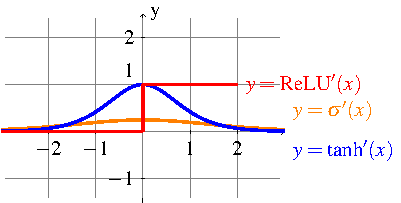
\includegraphics{\imgpath/nonlinearities_grad.pdf}
  \centering
  \mycaption{Common neural network nonlinearities and their gradients}{The sigmoid, tanh and ReLU
  nonlinearities are commonly used activation functions for neurons. The tanh
  and sigmoid have the nice property of being smooth but can have saturation
  when the input is either largely positive or largely negative, causing little
  gradient to flow back through it. The ReLU does not suffer from this problem
  and has the additional nice property of setting values to exactly 0, making a
  sparser output activation.}
  \label{fig:ch2:nonlinearities}
\end{figure}

\subsection{Multilayer Perceptrons}
As mentioned in the previous section, a single neuron can be thought of as a
separating hyperplane with an activation that maps the two halves of the space
to different values. Such a linear separator is limited and famously cannot
solve the XOR problem \cite{minsky_perceptrons:_1988}. Fortunately, adding a
single hidden layer like the one shown in \autoref{fig:ch2:hidden} can change
this, and it is proveable that with an infinitely wide hidden layer, a neural
network can approximate any function \cite{hornik_multilayer_1989,
cybenko_approximation_1989}. This extension is called a multilayer perceptron,
or MLP.

The forward pass of such a network with one hidden layer of $H$ units is:
%
\begin{align}
  h_i & =  \sigma\left(\sum_{j=0}^{D} x_j w_{ij}^{(1)}\right) \\
  y & =  \sum_{k=0}^{H} h_k w^{(2)}_{k}
\end{align}
%
where $w^{(l)}$ denotes the weights for the $l$-th layer, of which
\autoref{fig:ch2:hidden} has 2. Note that these individual layers are often
called \emph{fully connected} as each node in the previous layer affects every
node in the next.

If we were to expand this network to have $N_l$ such fully connected layers, we
could rewrite the action of each layer in a recursive fashion:
%
\begin{align}
  y^{(l+1)} &= W^{(l+1)}x^{(l)}  \label{eq:ch2:fc1}\\
  x^{(l+1)} &= \sigma\left(y^{(l+1)}\right) \label{eq:ch2:fc2}
\end{align}
where $W$ is now a weight matrix, acting on the vector of the previous layer's
outputs $x^{(l)}$. As we are now considering every layer to be an input to the next
stage, we have removed the $h$ notation and added the superscript $(l)$ to
define the depth. $x^{(0)}$ is the network input and $y^{(N_l)}$ is the network
output. Let us say that the output has $C$ nodes, and a hidden layer $x^{(l)}$
has $C_l$ nodes.

\begin{figure}[t]
  \centering
  % % MLP
\begin{tikzpicture}[scale=1]
    \def\nodedist{35pt}
    \def\layerdist{80pt}
    \def\pindist{20pt}
    
    \tikzstyle{every pin edge}=[signal]
    \tikzstyle{annot} = [text width=4em, text centered]
    
    \foreach \y in {1,...,3}
        \node[inputnode, pin={[pin edge={latex-}, pin distance=\pindist]left:Input \y}] 
            (I\y) at (0,-\y*\nodedist) {$x_\y$};  
    
    \foreach \y in {1,...,4}
        \node[hiddennode] 
            (H\y) at ($(\layerdist,-\y*\nodedist) +(0, 0.5*\nodedist)$) {$h_\y$};
    
    \foreach \y in {1,...,1}
        \node[outputnode, pin={[pin edge={-latex}, pin distance=\pindist]right:Output \y}]
            (O\y) at ($(I2) + (2*\layerdist, 0)$) {$y_\y$};
    
    \foreach \dest in {1,...,4}
        \foreach \source in {1,...,3}
            \draw[signal] (I\source) -- (H\dest);
    
    \foreach \dest in {1,...,1}
        \foreach \source in {1,...,4}
            \draw[signal] (H\source) edge (O\dest);
    
    \node[annot, above=4pt of H1] (hl) {Hidden layer};
    \node[annot] at (I1 |- hl) {Input layer};
    \node[annot] at (O1 |- hl) {Output layer};
\end{tikzpicture}

  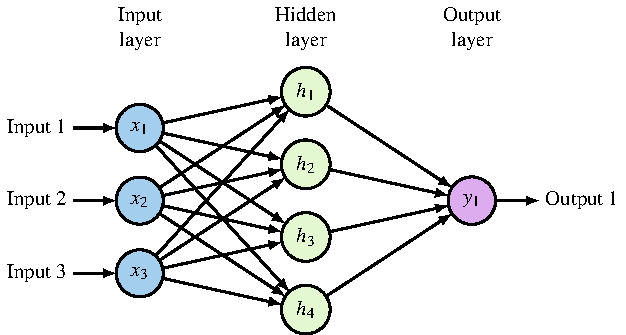
\includegraphics{\imgpath/network_mlp.pdf}
  \mycaption{Multi-layer perceptron}{Expanding the single neuron from
  \autoref{fig:ch2:singlelayer} to a network of neurons. The internal
  representation units are often referred to as the \emph{hidden layer} as they
  are an intermediary between the input and output.}
  \label{fig:ch2:hidden}
\end{figure}

\subsection{Backpropagation}
It is important to truly understand backpropagation when designing neural
networks, so we describe the core concepts now for a neural network with
$N_l$ layers.

The delta rule, initially designed for networks with no hidden layers
\cite{widrow_neurocomputing:_1988}, was expanded to what we now consider
\emph{backpropagation} in \cite{rumelhart_parallel_1986}. While backpropagation
is conceptually just the application of the chain rule, Rumelhart, Hinton, and
Williams successfully updated the delta rule to networks with hidden layers,
laying a key foundational step for deeper networks.

With a deep network, calculating $\dydx{L_{data}}{w}$ may not seem easy,
particularly if $w$ is a weight in one of the earlier layers. We need
to define a rule for updating the weights in all $N_l$ layers of the network,
$W^{(1)}, W^{(2)}, \ldots W^{(N_l)}$ however, only the final set $W^{(N_l)}$ are
connected to the data loss function $L_{data}$.

\subsubsection{Regression Loss}
Let us start with writing down the derivative of $L$ (dropping the \emph{data}
subscript for now) with respect to the network
output $\hat{y} = y^{(N_l)}$ using the regression objective function \eqref{eq:ch2:mle_reg}.
\begin{align}
  \dydx{L}{y^{(N_l)}} &= \dydx{}{\hat{y}} \left( \frac{1}{N}\sum_{n=1}^{N_b}\frac{1}{2} \left(y^{(n)} - \hat{y}^{(n)}\right)^2\right) \\
                    &= \frac{1}{N}\sum_{n=1}^{N_b} \left(\hat{y}^{(n)} - y^{(n)} \right) \\
                    &= e \in \reals \label{eq:ch2:reg_b1}
\end{align}
where we have used the fact that for the regression case, $y^{(n)},\ \hat{y}^{(n)}
\in \reals$.

\subsubsection{Classification Loss}
For the classification case \eqref{eq:ch2:mle_class}, let us keep the output of
the network as $y^{(N_l)} \in \reals[C]$ and define $\hat{y}$ as the
softmax applied to this vector $\hat{y}^{(n)}_c = \sigma_c\left(y^{(N_l, n)}\right)$.
As we now have two superscripts,
one for the sample number and one for the layer number, we combine them into a
tuple of superscripts.

Note that the softmax is a vector-valued function going from $\reals[C] \rightarrow
\reals[C]$ so has a Jacobian matrix $S$ with values:
\begin{equation}
  S_{ij} = \dydx{\hat{y}_i}{y^{(N_l)}_j} = \begin{cases}
    \sigma_i (1-\sigma_j) & \text{if $i=j$}\\
    -\sigma_i \sigma_j & \text{if $i\neq j$}\\
  \end{cases}
\end{equation}

Now, let us return to \eqref{eq:ch2:mle_class} and find the derivative of the
objective function to this output value $\hat{y}$:
\begin{align}
  \dydx{L}{\hat{y}} &=  \dydx{}{\hat{y}} \left( \frac{1}{N}\sum_{n=1}^{N_b} \sum_{c=1}^C
  y^{(n)}_c \log \hat{y}^{(n)}_c \right) \\
  &= \frac{1}{N}\sum_{n=1}^{N_b} \sum_{c=1}^C \frac{y^{(n)}_c}{\hat{y}^{(n)}_c} \\
  &= d \in \reals[C] \label{eq:ch2:class_b1}
\end{align}
Note that unlike \eqref{eq:ch2:reg_b1}, this derivative is vector-valued. To
find $\dydx{L}{y^{(N_l)}}$ we use the chain rule. It is easier to find the
partial derivative with respect to one node in the output first, and then expand
from here. I.e.:

\begin{align}
  \dydx{L}{y^{(N_l)}_j} &= \sum_{i=1}^C \dydx{L}{\hat{y}_i}\dydx{\hat{y}_i}{y^{(N_l)}_j} \\
                      &= S_j^T d
\end{align}
where $S_j$ is the $j$th column of the Jacobian matrix $S$. It becomes clear now
that to get the entire vector derivative for all nodes in $y^{(N_l)}$, we must
multiply the transpose of the Jacobian matrix with the error term from
\eqref{eq:ch2:class_b1}:
\begin{equation}
  \dydx{L}{y^{(N_l)}} = S^T d
\end{equation}

\subsubsection{Final Layer Weight Gradient} \label{sec:ch2:weight}
Let us continue by assuming $\dydx{L}{y^{(N_l)}}$ is vector-valued as was the case
with classification. For regression, it is easy to set $C=1$ in the following to
get the necessary results. For clarity we drop the layer
superscript in the intermediate calculations.

We call the gradient for the final layer weights the \emph{update} gradient.
It can be computed by the chain rule again:
\begin{align}
  \dydx{J}{W_{ij}} &= \dydx{L_{data}}{y_i} \dydx{y_i}{W_{ij}} + \lambda W_{ij} \\
                   &= \dydx{L_{data}}{y_i} x_j + \lambda W_{ij}
\end{align}
where the second term in the above two equations comes from the regularization
loss that is added to the objective. The update gradient of the entire weight matrix is
then:
\begin{align}
  \dydx{J}{W^{(N_l)}} &= \dydx{L_{data}}{\hat{y}} x^T +2\lambda W \\
                    &= S^T d \left(x^{(N_l-1)}\right)^T + 2\lambda W^{(N_l)} \in \reals[C \x C_{N_l-1}]
\end{align}

\subsubsection{Final Layer Passthrough Gradient} \label{sec:ch2:passthrough}
We also want to find the \emph{passthrough} gradients of the final
layer $\dydx{L}{x^{(N_l-1)}}$ (these are not affected by the regularization
terms, so we only need to find the gradient w.r.t. the data loss $L$). In a
similar fashion, we first find the gradient with respect to individual elements
in $x^{(N_l-1)}$ before generalizing to the entire vector:
\begin{align}
  \dydx{L}{x_i} &= \sum_{j=1}^{C} \dydx{L}{y_j} \dydx{y_j}{x_i} \\
                &= \sum_{j=1}^{C} \dydx{L}{y_j} W_{j,i} \\
                &= W_{i}^T\dydx{L}{y} \\
\end{align}
where $W_i$ is the $i$th column of $W$. Thus
\begin{align}
  \dydx{L}{x^{(N_l-1)}} &= \left(W^{(N_l)}\right)^T \dydx{L}{y^{(N_l)}} \\
                      &= \left( W^{(N_l)} \right)^T S^T d
\end{align}
This passthrough gradient then can be used to update the next layer's weights by
repeating \autoref{sec:ch2:weight} and \autoref{sec:ch2:passthrough}.

\subsubsection{General Layer Update}
The easiest way to handle this flow of gradients and the basis for most
automatic differentiation packages is the block definition shown in
\autoref{fig:ch2:block_form}. For all neural network components (even if they do
not have weights), the operation must not only be able to calculate the forward
pass $y=f(x, w)$ given weights $w$ and inputs $x$, but also calculate the
\emph{update} and \emph{passthrough} gradients $\dydx{L}{w}, \dydx{L}{x}$ given
an input gradient $\dydx{L}{y}$. The input gradient will have the same shape as
$y$ as will the update and passthrough gradients match the shape of $w$ and $x$.
This way, gradients for the entire network can be computed in an iterative
fashion starting at the loss function and moving backwards.

\begin{figure}
  \centering
  % \begin{tikzpicture}[every node/.style={node font=\large}]
\definecolor{mycolor}{RGB}{252,247,189};
\pgfmathsetmacro{\EDGE}{.5}
\node [fill=mycolor, draw, minimum width=3cm, minimum height=2cm] (block) at (1,1) {$y=f(x,w)$};
\coordinate[right=\EDGE of block.south west] (xin);
\coordinate[left=\EDGE of block.south east] (dxin);
\coordinate[below=\EDGE of block.north west] (win);
\coordinate[above=\EDGE of block.south west] (dwin);
\coordinate[right=\EDGE of block.north west] (yin);
\coordinate[left=\EDGE of block.north east] (dyin);
\draw[<-] (xin) -- +(0,-1) node[below] {$x$};
\draw[->] (dxin) -- ++(0,-1) node[below] {$\dydx{\logloss}{x}$};
\draw[<-] (win) -- ++(-1,0) node[left] {$w$};
\draw[->] (dwin) -- ++(-1,0) node[left] {$\dydx{\logloss}{w}$};
\draw[->] (yin) -- ++(0,1) node[above] {$y$};
\draw[<-] (dyin) -- ++(0,1) node[above] {$\dydx{\logloss}{y}$};
\end{tikzpicture}

  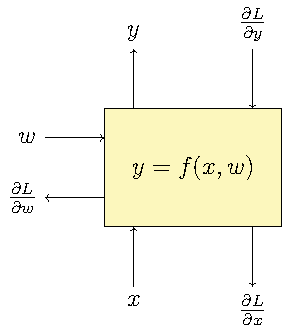
\includegraphics{\imgpath/deeplearn_block.pdf}
  \mycaption{General block form for autograd}{All neural network functions
  need to be able to calculate the forward pass $y=f(x,w)$ as well as the
  update and passthrough gradients $\dydx{L}{w}, \dydx{L}{x}$. Backpropagation
  is then easily done by allowing data to flow backwards through these blocks
  from the loss.}
  \label{fig:ch2:block_form}
\end{figure}

\section{Convolutional Neural Networks}\label{sec:ch2:cnns}
Convolutional Neural Networks (CNNs) are a special type of Neural Network built mainly from
\emph{convolutional layers} rather than fully connected layers. A convolutional
layer is one where the weights are shared spatially across the layer.
In this way, a neuron at is only affected by
nodes from the previous layer in a given neighbourhood, rather than from every node.

First popularized in 1998 by LeCun et.\ al.\ in \cite{lecun_gradient-based_1998},
the convolutional layer was introduced to build invariance with respect to
translations, as well as reduce the parameter size of early neural networks for
pattern recognition. The idea of having a locally-receptive field had already
been shown to be a naturally occurring phenomenon by Hubel and Wiesel
\cite{hubel_receptive_1962}. They did not become popular immediately, and
another spatially based keypoint extractor, SIFT \cite{lowe_distinctive_2004},
was the mainstay of detection systems until the AlexNet CNN
\cite{krizhevsky_imagenet_2012} won the 2012 ImageNet challenge
\cite{russakovsky_imagenet_2015-1} by a large margin over the next competitors, many of
whom used SIFT\@. This CNN had 5 convolutional layers followed by 3 fully
connected layers.

We now briefly describe the convolutional layer, as well as many other layers
used in CNNs that have become popular in the past few years.

\subsection{Convolutional Layers}\label{sec:ch2:conv_layers}
In the analysis of neural networks so far, we have considered column vectors
$x^{(l)},y^{(l)} \in \reals[C_{l}]$. Convolutional layers for image analysis
have a different format, with the spatial component of the input is
preserved.

Let us first consider the definition of 2-D convolution for single-channel
images:
\begin{align}
  y[\nn] = (x\conv h)[\nn] &= \sum_{\kk} x[\kk]h[\nn-\kk] \label{eq:ch2:conv1}\\
                           &= \sum_{k_1, k_2} x[k_1,k_2]h[n_1-k_1, n_2-k_2]
\end{align}
where the sum is done over the support of $h$. For an input $x\in \reals[H\x W]$
and filter $h\in \reals[K_H\x K_W]$ the output has spatial support $y\in
\reals[H+K_H-1 \x W+K_W-1]$.

The filter $h$ can also be thought of as a \emph{matched filter}
that gives its largest output when the input contains the mirror of $h$, $\tilde{h}$. If the input has
shapes similar to $\tilde{h}$ in many locations, each of these locations in $y$ will
also have large outputs.

If we stack red, green and blue input channels on top of each other\footnote{In deep
learning literature, there is not a consensus about whether to stack the outputs
with the channel first ($\reals[C\x H\x W]$) or last ($\reals[H\x W\x C]$). The
latter is more common in Image Processing for colour and spectral images but
the former is the standard for many deep learning frameworks, including the one
we use -- PyTorch \cite{paszke_automatic_2017}. For this reason, we stack
channels along the first dimension of our tensors.}, we have a
3-dimensional input $x \in \reals[C\x H\x W]$ with $C=3$.
This third dimension is often called the \emph{depth} dimension, to distinguish
it from the two spatial dimensions. In a CNN layer, each filter $h$ is three
dimensional with depth exactly equal to $C$. The convolution is
done only over the two spatial dimensions
and the $C$ outputs are summed at each pixel location. This makes
\eqref{eq:ch2:conv1}:
\begin{equation}
  y[\nn] = \sum_{c=0}^{C-1} \sum_{\kk} x[c, \kk]h[c, \nn-\kk]
  \label{eq:ch2:conv2}
\end{equation}

It is not enough to only have a single matched filter and often we would like to
have a bank of them, each one sensitive to a different shape. For example, if
one filter is sensitive to horizontal edges, we may also want to detect vertical, and
diagonal edges. Let us rename the number of channels in the input layer as
$C_{l}$ and specify that we would like to have $C_{l+1}$ different matched
filters. We then stack each of the single-channel outputs from
\eqref{eq:ch2:conv2} to give the output $y \in \reals[C_{l+1} \x H\x W]$:
%
\begin{equation}
  y[f, \nn] = \sum_{c=0}^{C-1} \sum_{\kk} x[c, \kk]h[f, c, \nn-\kk]
  \label{eq:ch2:conv3}
\end{equation}

After a convolutional layer, we can then apply a pointwise nonlinearity to
each output location in $y$. Like multilayer perceptrons, this was typically the
sigmoid function $\sigma$, but is now more commonly the ReLU\@. Revisiting
\eqref{eq:ch2:fc1} and
\eqref{eq:ch2:fc2}, we can rewrite this for a convolutional layer at depth $l$
with $C_l$ input and $C_{l+1}$ output channels:
\begin{align}
  y^{(l+1)}[f, \nn] &= \sum_{c=0}^{C_l-1} x^{(l)}[c, \nn] \conv h^{(l)}[f, c, \nn]
    \label{eq:ch2:conv4}\\
    x^{(l+1)}[f, \nn] &= \sigma\left(y^{(l)}[f, \nn]\right) \label{eq:ch2:conv4a}
\end{align}
where $f \in \{0, 1,\ldots C_{l+1}-1\}$ indexes the filter number/output channel. A diagram
representing this operation is shown in \autoref{fig:ch2:conv_layer}.

\begin{figure}
  \centering
  %   \begin{tikzpicture}[%
    path image/.style={
      path picture={
        \node at (path picture bounding box.center) {
          \includegraphics[height=2.0cm]{#1}
        };
      }
    }, 
    path pic/.style={
      path picture={
        \node at (path picture bounding box.center) {
          \includegraphics[height=1.2cm]{#1}
        };
      }
    }, 
    path pic2/.style={
      path picture={
        \node at (path picture bounding box.center) {
          \includegraphics[height=0.8cm]{#1}
        };
      }
    }, 
    scale=0.8]

    \tikzcuboid{
    shiftx=0cm,
    shifty=-1cm,
    scale=0.5,
    dimx=2, dimy=2, dimz=12,
    densityx=2, densityy=2, densityz=2,
    dimxval=W, dimyval=H, dimzval=C_l,
    drawxdims=true, drawydims=true, drawzdims=true,
    front/.style={draw=blue!50!white,fill=blue!50!white},%
    right/.style={draw=blue!50!white,fill=blue!50!white},%
    top/.style={draw=blue!50!white,fill=blue!50!white},%
    shade=false,
    emphedge=true,
    shadeopacity=0,
    emphstyle/.style={rounded corners=0.2pt,line width=0.3mm},
    }
    \draw (1.6, 1.7, 0) node {\large{$x^{(l)}$}};
    \draw (5.5, 2.9, 0) node {\large{$h^{(l+1)}$}};
    \draw (9.7, 1.6, 0) node {\large{$y^{(l+1)}$}};
    \draw (13.7, 1.6, 0) node {\large{$x^{(l+1)}$}};
    \draw (2.2, -.8, 0) node {\Large{$\conv$}};

    \tikzcuboid{
    shiftx=4cm,
    shifty=1cm,
    scale=0.5,
    dimx=.7, dimy=.7, dimz=12,
    dimxval=k_w, dimyval=k_h,
    densityx=5, densityy=5, densityz=2,
    drawxdims=false,
    drawydims=false,
    drawzdims=false,
    front/.style={draw=red!50!white,fill=red!50!white},%
    right/.style={draw=red!50!white,fill=red!50!white},%
    top/.style={draw=red!50!white,fill=red!50!white},%
    }
    \tikzcuboid{
    shifty=0cm,
    }
    \tikzcuboid{
    shifty=-2.0cm,
    scale=0.5,
    drawxdims=true,
    drawydims=true,
    drawzdims=true,
    dimzval=C_l,
    }
    \draw (3.2, -1.7, -2.8) node {$\vdots$};
    \draw [<->] (3.3, 0.1, -6) -- (3.3, -3.2, -6) node[near start, right] {$C_{l+1}$};
    \draw [->, fill=gray!30,ultra thick] (5, -1.5, -2.5) -- (6, -1.5, -2.5);

    \tikzcuboid{
    shiftx=8cm,
    shifty=-1cm,
    scale=0.5,
    dimx=2, dimy=2, dimz=10,
    densityx=4, densityy=4, densityz=2,
    dimzval=C_{l+1},
    drawzdims=true,
    drawxdims=false,
    drawydims=false,
    front/.style={draw=blue!50!white,fill=blue!50!white},%
    right/.style={draw=blue!50!white,fill=blue!50!white},%
    top/.style={draw=blue!50!white,fill=blue!50!white},%
    }
    \draw [->, fill=gray!30,ultra thick] (9, -1.5, -2.5) -- (10, -1.5, -2.5)
      node[midway, above] {$g$};

    \tikzcuboid{
    shiftx=12cm,
    shifty=-1cm,
    scale=0.5,
    dimx=2, dimy=2, dimz=10,
    densityx=4, densityy=4, densityz=2,
    drawzdims=true,
    dimzval=C_{l+1},
    drawxdims=false,
    drawydims=false,
    drawzdims=false,
    front/.style={draw=blue!50!white,fill=blue!50!white},%
    right/.style={draw=blue!50!white,fill=blue!50!white},%
    top/.style={draw=blue!50!white,fill=blue!50!white},%
    }

  \end{tikzpicture}

  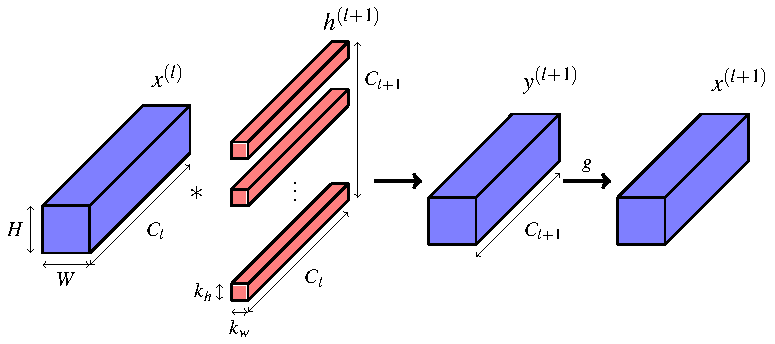
\includegraphics[width=\textwidth]{\imgpath/conv.pdf}
  \mycaption{A convolutional layer}{A convolutional layer followed by a
  nonlinearity $\sigma$. The previous layer's activations are convolved with a bank
  of $C_{l+1}$ filters, each of which has spatial size $k_h\x k_w$ and depth
  $C_l$. Note that there is no convolution across the channel dimension. Each
  filter produces one output channel in $y^{(l+1)}$.}
  \label{fig:ch2:conv_layer}
\end{figure}

\subsubsection{Padding and Stride}\label{sec:ch2:padding}
Regular 2-D convolution expands the input from size $H\x W$ to $(H+K_H-1)\x
(W+K_W-1)$. In neural networks, this is called \emph{full convolution}.
It is often desirable (and common) to
have the same output size as input size, which can be achieved by
taking the central $H\x W$ outputs of full convolution. This is often
called \emph{same-size convolution}.
Another option commonly used is to only evaluate the kernels where they fully
overlap the input signal, causing a reduction in the output size to $(H-K_H+1)
\x (W-K_W+1)$. This is called \emph{valid convolution} and was used in the
original LeNet-5 \cite{lecun_gradient-based_1998}.

Signal extension for full and same-size convolution is by default \emph{zero
padding}, and most deep learning frameworks have no ability to choose other
padding schemes as part of their convolution functions. Other padding such as
\emph{symmetric padding} can be achieved by expanding the input signal before
doing a valid convolution.

\emph{Stride} is a commonly used term in deep learning literature. A stride of 2 means
that we evaluate the filter kernel at every other input location. In signal
processing, this is simply called decimation by 2.

\subsubsection{Gradients}\label{sec:ch2:conv_grad}
To get the update and passthrough gradients for the convolutional layer we will need to expand
\eqref{eq:ch2:conv4} (again we will drop the layer superscripts for clarity):
\begin{equation}
  % Y[f, n_1, n_2] &=& \sum_{c=1}^C \sum_{k_1=a}^{b} \sum_{k_2=a}^b x[c, k_1, k_2]
  % h_f[c, n_1-k_1, n_2-k_2] \label{eq:ch2:conv5}
  y[f, n_1, n_2] = \sum_{c=0}^{C-1} \sum_{k_1} \sum_{k_2} x[c, k_1, k_2]
  h[f, c, n_1-k_1, n_2-k_2] \label{eq:ch2:conv5}
\end{equation}
The derivative for a single output $y[f, n_1, n_2]$ w.r.t.\ a single input $x[c, k_1, k_2]$ is then
simply:
\begin{equation}
  \dydx{y_{f, n_1, n_2}}{x_{c, k_1, k_2}} = h[f, c, n_1 - k_1, n_2 - k_2]
\end{equation}
It is clear from \eqref{eq:ch2:conv5} that a single activation $x[c, k_1, k_2]$ affects
many output values. Thus, the derivative for the loss function to this single
point in $x$ is the sum of the chain rule applied to all output positions:
\begin{align}
  \dydx{L}{x_{c,k_1,k_2}} &= \sum_f \sum_{n_1} \sum_{n_2} \dydx{L}{y_{f, n_1, n_2}}
  \dydx{y_{f, n_1, n_2}}{x_{c,k_1,k_2}} \\
  &= \sum_f \sum_{n_1} \sum_{n_2} \dydx{L}{y_{f, n_1, n_2}} h[f, c, n_1 - k_1, n_2 - k_2] \label{eq:ch2:conv6}
\end{align}
Now we let $\Delta y[f, n_1, n_2] = \dydx{L}{y_{f, n_1, n_2}}$ be the passthrough gradient
signal from the next layer, and $\tilde{h}[\alpha, \beta, \gamma, \delta] = h[\beta, \alpha, -\gamma, -\delta]$
be a set of filters that have been mirror-imaged in the spatial domain and had
their filter and channel dimensions transposed. Combining these two and
substituting into \eqref{eq:ch2:conv6}, we get the passthrough gradient for the
convolutional layer:
\begin{align}
  \dydx{L}{x_{c,k_1,k_2}} &= \sum_f \sum_{n_1} \sum_{n_2} \Delta y[f, n_1, n_2] \tilde{h}[c, f, k_1-n_1, k_2-n_2 ] \\
                          &= \sum_f \Delta y[f, \kk] \conv \tilde{h}[c, f, \kk] \label{eq:ch2:cnn_passthrough}
\end{align}
which is the same as \eqref{eq:ch2:conv4}. I.e.\ we can backpropagate the
gradients through a convolutional layer by mirror-imaging the filters spatially,
transposing them in the channel and filter dimensions, and doing a forward
convolutional layer with $\tilde{h}$ applied to $\Delta y$. Similarly, we
find the update gradients to be:
\begin{align}
  \dydx{L}{h_{f,c,k_1,k_2}} &= \sum_{n_1} \sum_{n_2} \dydx{L}{y_{f, n_1, n_2}} \dydx{y_{f, n_1, n_2}}{h_{f, c, k_1, k_2}}  \\
                            &= \sum_{n_1} \sum_{n_2} \Delta y[f, n_1, n_2] x[c, n_1-k_1, n_2-k_2 ] \\
                            &= \left(\Delta y[f] \star x[c]\right)[k_1, k_2] \label{eq:ch2:cnn_weight_update}
\end{align}
where $\star$ is the cross-correlation operation.

\subsection{Pooling}
\emph{Pooling} layers are common in CNNs where we want to reduce the spatial size. As
we go deeper into a CNN, it is common for the spatial size of the activation to
decrease, and the channel dimension to increase. The $C_l$ values at a given
spatial location can then be thought of as a feature vector describing the
presence of shapes in a given area in the input image.

Pooling is useful to add some invariance to smaller shifts when downsampling. It
is often done over small spatial sizes, such as $2\x 2$ or $3\x 3$. Invariance
to larger shifts can be built up with multiple pooling (and convolutional) layers.

Two of the most common pooling techniques are \emph{max pooling} and
\emph{average pooling}. Max pooling takes the largest value in its spatial area,
whereas average pooling takes the mean. A visual explanation is shown in
\autoref{fig:ch2:maxpool}. Note that pooling is typically a spatial operation,
and only in rare cases is done over the channel/depth dimension.

A review of pooling methods in \cite{mishkin_systematic_2017} found both
max and average pooling to perform similarly well. While max pooling was the most
popular in earlier state of the art networks \cite{krizhevsky_imagenet_2012,
simonyan_very_2014}, there has been a recent trend towards using average pooling
\cite{huang_densely_2017} or even to do away with pooling altogether in favour
of strided convolutions (this idea was originally proposed in
\cite{springenberg_striving_2015} and used notably in \cite{he_deep_2016,
xie_aggregated_2017, zagoruyko_wide_2016}).

\begin{figure}
  \centering
  % % max and average pooling, kernel (2,2), stride (2,2)

\begin{tikzpicture}
    \coordinate (p) at (0,0);
    \draw[shift={(p)}, fill=red!20!white] (0,0) rectangle (2,-2);
    \draw[shift={(p)}, fill=yellow!20!white] (2,0) rectangle (4,-2);
    \draw[shift={(p)}, fill=blue!20!white] (0,-2) rectangle (2,-4);
    \draw[shift={(p)}, fill=green!20!white] (2,-2) rectangle (4,-4);
    \draw[
        ultra thick,
        step=1, 
        color=black,
        draw=black,
        fill=black!20!white,
        shift={(p)}
    ] (0,0) grid (4,-4)
    foreach[count=~] \l in {73, 74, 17, 49, 10, 29, 41, 20, 4, 23, 39, 4, 50, 80, 56, 57} {
        ({0.5+mod(~-1,4}, {-0.5-div(~-1,4}) node {\Large \l}
    };
    
    % max pooling
    \coordinate (p) at (7,0.5);
    \draw[shift={(p)}, fill=red!20!white] (0,0) rectangle (1,-1);
    \draw[shift={(p)}, fill=yellow!20!white] (1,0) rectangle (2,-1);
    \draw[shift={(p)}, fill=blue!20!white] (0,-1) rectangle (1,-2);
    \draw[shift={(p)}, fill=green!20!white] (1,-1) rectangle (2,-2);
    \draw[
        ultra thick,
        step=1, 
        color=black,
        draw=black,
        fill=black!20!white,
        shift={(p)}
    ] (0,0) grid (2,-2)
    foreach[count=~] \l in {74, 49, 80, 57} {
        ({0.5+mod(~-1,2}, {-0.5-div(~-1,2}) node {\Large \l}
    };
    \draw[signal] (4.5,-1.5) -> ($(p) +(-0.5, -1.25)$);
    \node[text width=200pt, align=center, right of=p, yshift=10pt] (l1) {Max Pooling};
    
    % average pooling
    \coordinate (p) at (7,-2.5);
    \draw[shift={(p)}, fill=red!20!white] (0,0) rectangle (1,-1);
    \draw[shift={(p)}, fill=yellow!20!white] (1,0) rectangle (2,-1);
    \draw[shift={(p)}, fill=blue!20!white] (0,-1) rectangle (1,-2);
    \draw[shift={(p)}, fill=green!20!white] (1,-1) rectangle (2,-2);
    \draw[
        ultra thick,
        step=1, 
        color=black,
        draw=black,
        fill=black!20!white,
        shift={(p)}
    ] (0,0) grid (2,-2)
    foreach[count=~] \l in {46, 32, 39, 39} {
        ({0.5+mod(~-1,2}, {-0.5-div(~-1,2}) node {\Large \l}
    };
    \draw[signal] (4.5,-2.5) -> ($(p) +(-0.5, -0.75)$);
    \node[text width=200pt, align=center, right of=p, yshift=10pt] (l1) {Average Pooling};
\end{tikzpicture}
  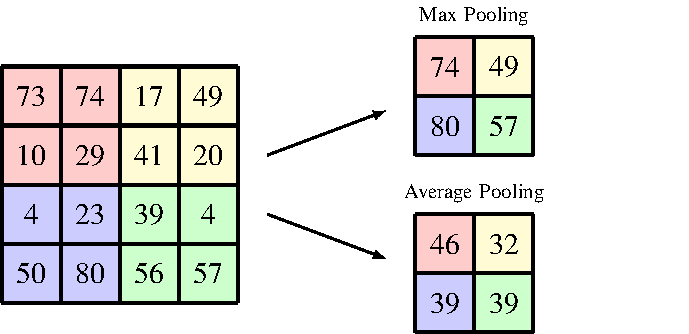
\includegraphics{\imgpath/pooling_both.pdf}
  \mycaption{Max vs Average $2\x 2$ pooling}{}
  \label{fig:ch2:maxpool}
\end{figure}

\subsection{Dropout}
\emph{Dropout} is a particularly strong regularization scheme that randomly turns off,
or `zeros out', neurons in a neural network \cite{hinton_improving_2012, srivastava_dropout:_2014}.
Each neuron has probability $p$ of having its value set to 0 (independently of
other neurons) during training
time, forcing the network to be more general and preventing `co-adaption' of
neurons \cite{srivastava_dropout:_2014}.

During test time, dropout is typically turned off, but can still be
used to get an estimate on the uncertainty of the network by averaging over
several runs \cite{gal_dropout_2016}.

\subsection{Batch Normalization}
\emph{Batch normalization} proposed in \cite{ioffe_batch_2015} is a conceptually
simple technique which rescales activations of a neural network. Despite its
simplicity, it has become very popular and has been found to be very useful to
train deeper CNNs.

First let us define $\mu_c^{(l)}$ and $\sigma_c^{(l)}$ as the mean and standard deviations
for a channel in a given activation at layer $l$. This mean and standard deviation is taken by
averaging across the entire dataset (with $N$ samples), and at every spatial location.
\begin{align}
  \mu_c^{(l)} &= \frac{1}{N}\sum_{i=0}^{N-1} \sum_\nn x^{(l, i)}[c, \nn] \\
  (\sigma_c^{(l)})^2 &=  \frac{1}{N} \sum_{i=0}^{N-1} \sum_\nn \left(x^{(l, i)}[c, \nn]\right)^2 - (\mu^{(l)}_c)^2
\end{align}
where $\mu, \sigma \in \reals[C]$.
Batch normalization removes the mean and variance of the data, scales the data
by a learnable gain $\gamma$ and shifts the data to a learnable mean $\beta$,
with $\gamma, \beta \in \reals[C]$. If we drop the layer superscripts, this
means the action of batch normalization is defined by:
\begin{equation}
  y[c, \nn] = \frac{x[c, \nn] - \mu_c}{\sigma_c + \epsilon}\gamma_c + \beta_c
\end{equation}
where $\epsilon$ is a small value to avoid dividing by 0.

Of course, during training, we do not have access to the dataset statistics $\mu, \sigma$
so these values are estimated from the batch statistics. A typical practice
is to keep an exponential moving average estimate of these values.

The passthrough and update gradients are:
\begin{align}
  \dydx{L}{x_{c, n_1, n_2}} &= \dydx{L}{y_{c, n_1, n_2}}\frac{\gamma}{\sigma + \epsilon}\\
  \dydx{L}{\beta_c} &=  \sum_\nn \dydx{L}{y_{c, \nn}}\\
  \dydx{L}{\gamma_c} &= \sum_\nn \dydx{L}{y_{c, \nn}}\frac{x_{c, \nn} - \mu_c}{\gamma_c + \epsilon}
\end{align}

Batch normalization layers are typically placed \emph{between} convolutional layers
and nonlinearities.

Consider a linear operation such as convolution with weights $W$ acting on the
previous layer's output $X$, defined by $Y = WX$.
Batch normalization
removes the sensitivity of our network to
initial scaling of the weights, as
$BN(aWX) = BN(WX)$.
It is also particularly useful for backpropagation as an increase in weight
scale does not change the passthrough gradients and leads to \emph{smaller}
update gradients \cite{ioffe_batch_2015}, making the network more resilient to
the problems of vanishing and exploding gradients:
\begin{align}
  \frac{\partial BN((aW)X)}{\partial X} & =  \frac{\partial
  BN(WX)}{\partial X} \nonumber\\
  \frac{\partial BN((aW)X)}{\partial (aW)} & =  \frac{1}{a} \cdot \frac{\partial
  BN(WX)}{\partial W}
\end{align}

\section{Relevant Architectures and Datasets}
In this section, we briefly review some relevant CNN architectures that will be
helpful to refer back to in this thesis.

\subsection{Datasets}
When doing image analysis tasks it is important to know comparatively how well
different networks perform on the same challenge. To achieve this, the
community has developed several datasets that are commonly used to report
metrics. For image classification there are five such datasets, listed here in
increasing order of difficulty:
\begin{enumerate}
  \item \textbf{MNIST}: 10 classes, 6000 images per class, $28\x 28$ pixels per image.
    The images contain the digits 0--9 in greyscale on a blank background. The
    digits have been size normalized and centred. Dataset description and files can be obtained
    at \cite{lecun_modified_1998}.
  \item \textbf{CIFAR-10}: 10 classes, 5000 images per class, $32\x 32$ pixels per image.
    The images contain classes of everyday objects like cars, dogs, planes etc.
    The images are colour and have little clutter or background. Dataset
    description can be found in \cite{krizhevsky_learning_2009} and files at
    \cite{krizhevsky_cifar_2009}.
  \item \textbf{CIFAR-100}: 100 classes, 500 images per class, $32\x 32$ pixels per image.
    Similar to CIFAR-10, but now with fewer images per class and ten times as
    many classes. Dataset description can be found in
    \cite{krizhevsky_learning_2009} and files at \cite{krizhevsky_cifar_2009}.
  \item \textbf{Tiny ImageNet}: 200 classes, 500 images per class,
    $64 \x 64$ pixels per image. A more recently introduced dataset that bridges
    the gap between CIFAR and ImageNet. Images are larger than CIFAR and there
    are more categories. Dataset description and files can be obtained at \cite{li_tiny_2017}.
  \item \textbf{ImageNet CLS}: There are multiple types of challenges in ImageNet, but CLS
    is the classification challenge and is most commonly reported in papers.
    It has 1000 classes of objects with a varying amount of images per class.
    Most classes have 1300 examples in the training set, but a few have less
    than 1000. The images have variable size, typically a couple of hundred
    pixels wide and a couple of hundred pixels high. The images can have varying
    amounts of clutter and can be at different scales, making it a particularly
    difficult challenge. Dataset description is in
    \cite{russakovsky_imagenet_2015-1} and the most reliable source of the data
    can be found at \cite{stanford_vision_lab_imagenet_2017}.
\end{enumerate}
Several other classification datasets do exist but are not commonly used, such
as PASCAL VOC \cite{Everingham15} and Caltech-101 and Caltech-256
\cite{li_fei-fei_learning_2004}\footnote{Tiny ImageNet is also not commonly
used as it is quite new. We have included it in the main list as we have found it
to be quite a useful step up from CIFAR without requiring the weeks to train
experimental configurations on ImageNet.}.

\subsection{LeNet}
LeNet-5 \cite{lecun_gradient-based_1998} is a good network to start with: it
is simple yet contains many of the layers used in modern CNNs. Shown in
\autoref{fig:ch2:lenet} it has two convolutional and three fully connected
layers. The outputs of the convolutional layers are passed through a sigmoid
nonlinearity and downsampled with average pooling. The first two fully-connected
layers also have sigmoid nonlinearities. The loss function used is a combination
of tanh functions and MSE loss.

\begin{figure}
  \centering
  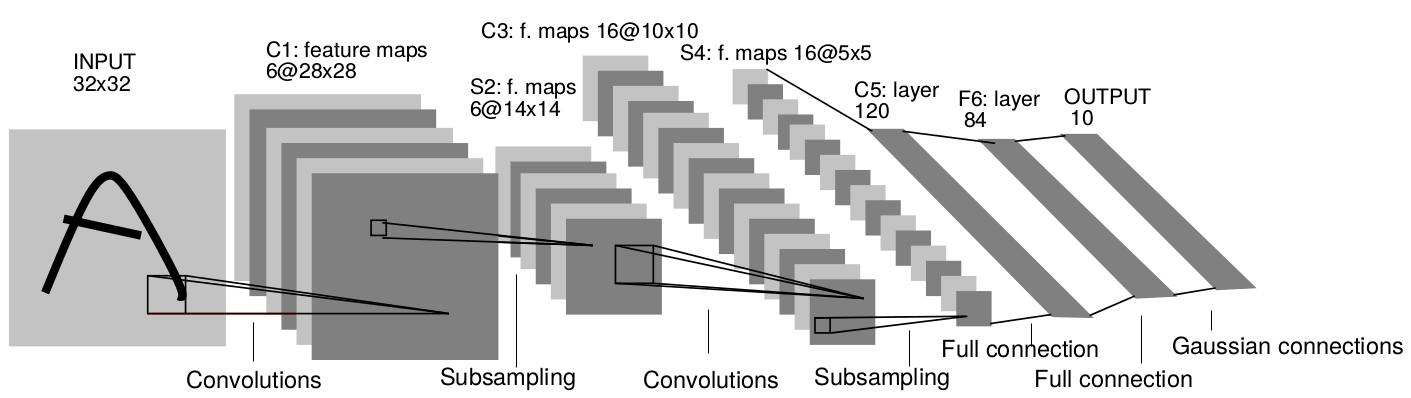
\includegraphics[width=\textwidth]{\imgpath/cnns.png}
  \mycaption{LeNet-5 architecture}{The `original' CNN architecture used for
  handwriting recognition. LeNet has 2 convolutional and 3 fully connected
  layers making 5 parameterized layers. After the second convolutional layer,
  the $16\x 5\x 5$ pixel output is unravelled to a $400$ long vector. Image
  is taken from \cite{lecun_gradient-based_1998}.}
  \label{fig:ch2:lenet}
\end{figure}

\subsection{AlexNet}
We have already seen AlexNet \cite{krizhevsky_imagenet_2012} in \autoref{ch:intro}.
It is arguably one of the most important architectures in the development in CNNs as it
was able to experimentally prove that CNNs can be used for complex tasks. This
required a few innovations: they used multiple GPUs to do fast
processing on large images, they used the ReLU to avoid saturation, and also added dropout
to aid generalization. Training of AlexNet on 2 GPUs available in 2012 takes
roughly a week.

The first layer uses convolutions with spatial support of $11\x11$, followed
by $5\x 5$ and $3\x 3$ for the final three layers.

% \begin{figure}
  % \centering
  % 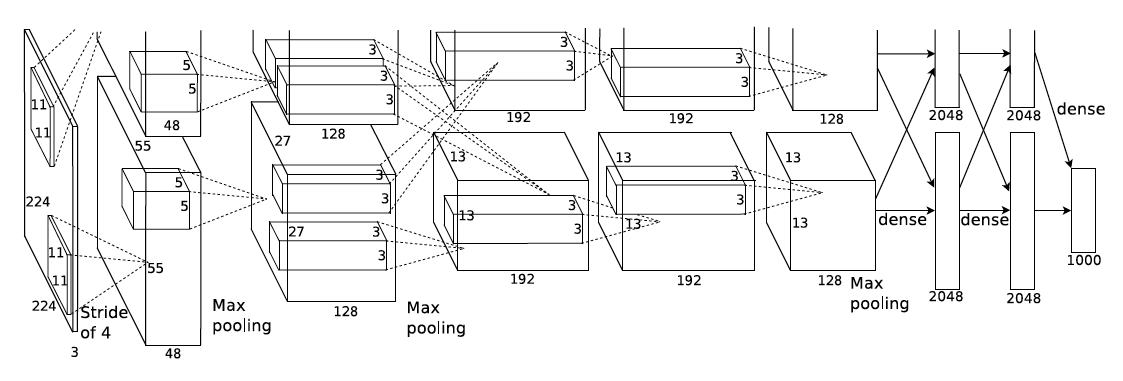
\includegraphics[width=\textwidth]{\imgpath/alexnet}
  % \mycaption{The AlexNet architecture}{Designed for the ImageNet challenge,
  % AlexNet may look like \autoref{fig:ch2:lenet} but is
  % much larger. Composed of 5 convolutional layers and 3 fully connected layers.
  % Figure taken from \cite{krizhevsky_imagenet_2012}.}
  % \label{fig:ch2:alexnet}
% \end{figure}

\subsection{VGGnet}
The Visual Geometry Group (VGG) at Oxford came second in the ILSVRC challenge in
2014 with their VGG-nets \cite{simonyan_very_2014}, but remains an important
network for some of the design choices it inspired. Their optimal
network was much deeper than AlexNet, with 19 convolutional layers on top of
each other before 3 fully connected layers. These convolutional layers all used
the smaller $3\x 3$ seen only at the back of AlexNet.

This network is particularly attractive due to its simplicity, compared to the
more complex Inception Network \cite{szegedy_going_2015} which won the 2014
ILSVRC challenge. VGG-16, the 16 layer variant of VGG stacks two or three
convolutional layers (and ReLUs) on top of each other before reducing spatial
size with max pooling. After processing at five scales, the resulting $512 \x 14
\x 14$ activation is unravelled and passed through a fully connected layer.

These VGG networks also marked the start of a trend that has since become
common, where channel depth is doubled after pooling layers. The doubling of
channels and quartering the spatial size still causes a net reduction in the
number of activations.

\subsection{The All Convolutional Network}
The All Convolutional Network \cite{springenberg_striving_2015} introduced two
popular modifications to the VGG networks:
%
\begin{itemize}
  \item They argued for the removal of max pooling layers, saying that a $3\x 3$
    convolutional layer with stride 2 works just as well.
  \item They removed the fully connected layers at the end of the network,
    replacing them with $1\x 1$ convolutions. Note that a $1\x 1$ convolution
    still has shared weights across all spatial locations. The output layer then
    has size $C_L \x H \x W$, where $H, W$ are many times smaller than the input
    image size, and the vector of $C_L$ coefficients at each spatial location
    can be interpreted as a vector of scores marking the presence/absence of
    $C_L$ different shapes. For classification, the output can be averaged over
    all spatial locations, whereas for localization it may be useful to keep
    this spatial information.
\end{itemize}
The new network was able to achieve state of the art results on CIFAR-10 and
CIFAR-100 and competitive performance on ImageNet, while only use a fraction of
the parameters of other networks.

\subsection{Residual Networks}\label{sec:ch2:resnets}
  \begin{figure}[tb]
    \centering
    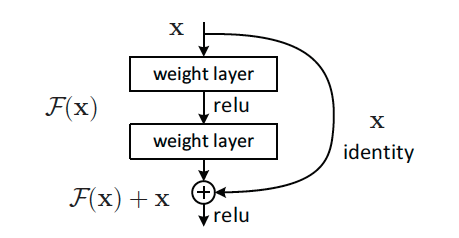
\includegraphics[width=0.5\textwidth]{\imgpath/residual_unit.png}
    \mycaption{The residual unit from ResNet}
          {A residual unit. The identity mapping is always present, and the
            network learns the difference from the identity mapping, $\mathcal{F}(x)$.
            Taken from \cite{he_deep_2016}.}
      \label{fig:ch2:residual_unit}
  \end{figure}
  Residual Networks or ResNets won the 2015 ILSVRC challenge, introducing the
  residual layer. Most state of the art models today use this residual mapping
  in some way \cite{zagoruyko_wide_2016, xie_aggregated_2017}.

  The inspiration for the residual layer came from the difficulties
  experienced in training deeper networks. Often, adding an extra layer would
  \emph{decrease} network performance. This is counter-intuitive as the deeper
  layers could simply learn the identity mapping, and achieve the same
  performance.

  To promote the chance of learning the identity mapping, they define a residual
  unit, shown in \autoref{fig:ch2:residual_unit}. If a desired mapping is
  denoted $\mathcal{H}(x)$, instead of trying to learn this, they instead learn
  $\mathcal{F}(x) = \mathcal{H}(x) - x$. Doing this promotes a strong diagonal
  in the Jacobian matrix which improves conditioning for gradient descent.

  Recent analyses of a ResNet without nonlinearities
  \cite{bartlett_representing_2018, bartlett_gradient_2018} proves that SGD
  fails to converge for deep networks when the network mapping is far away from
  the identity, suggesting that a residual mapping is a good thing to do.
